% Options for packages loaded elsewhere
\PassOptionsToPackage{unicode}{hyperref}
\PassOptionsToPackage{hyphens}{url}
%
\documentclass[
]{book}
\usepackage{amsmath,amssymb}
\usepackage{lmodern}
\usepackage{iftex}
\ifPDFTeX
  \usepackage[T1]{fontenc}
  \usepackage[utf8]{inputenc}
  \usepackage{textcomp} % provide euro and other symbols
\else % if luatex or xetex
  \usepackage{unicode-math}
  \defaultfontfeatures{Scale=MatchLowercase}
  \defaultfontfeatures[\rmfamily]{Ligatures=TeX,Scale=1}
\fi
% Use upquote if available, for straight quotes in verbatim environments
\IfFileExists{upquote.sty}{\usepackage{upquote}}{}
\IfFileExists{microtype.sty}{% use microtype if available
  \usepackage[]{microtype}
  \UseMicrotypeSet[protrusion]{basicmath} % disable protrusion for tt fonts
}{}
\makeatletter
\@ifundefined{KOMAClassName}{% if non-KOMA class
  \IfFileExists{parskip.sty}{%
    \usepackage{parskip}
  }{% else
    \setlength{\parindent}{0pt}
    \setlength{\parskip}{6pt plus 2pt minus 1pt}}
}{% if KOMA class
  \KOMAoptions{parskip=half}}
\makeatother
\usepackage{xcolor}
\usepackage{color}
\usepackage{fancyvrb}
\newcommand{\VerbBar}{|}
\newcommand{\VERB}{\Verb[commandchars=\\\{\}]}
\DefineVerbatimEnvironment{Highlighting}{Verbatim}{commandchars=\\\{\}}
% Add ',fontsize=\small' for more characters per line
\usepackage{framed}
\definecolor{shadecolor}{RGB}{248,248,248}
\newenvironment{Shaded}{\begin{snugshade}}{\end{snugshade}}
\newcommand{\AlertTok}[1]{\textcolor[rgb]{0.94,0.16,0.16}{#1}}
\newcommand{\AnnotationTok}[1]{\textcolor[rgb]{0.56,0.35,0.01}{\textbf{\textit{#1}}}}
\newcommand{\AttributeTok}[1]{\textcolor[rgb]{0.77,0.63,0.00}{#1}}
\newcommand{\BaseNTok}[1]{\textcolor[rgb]{0.00,0.00,0.81}{#1}}
\newcommand{\BuiltInTok}[1]{#1}
\newcommand{\CharTok}[1]{\textcolor[rgb]{0.31,0.60,0.02}{#1}}
\newcommand{\CommentTok}[1]{\textcolor[rgb]{0.56,0.35,0.01}{\textit{#1}}}
\newcommand{\CommentVarTok}[1]{\textcolor[rgb]{0.56,0.35,0.01}{\textbf{\textit{#1}}}}
\newcommand{\ConstantTok}[1]{\textcolor[rgb]{0.00,0.00,0.00}{#1}}
\newcommand{\ControlFlowTok}[1]{\textcolor[rgb]{0.13,0.29,0.53}{\textbf{#1}}}
\newcommand{\DataTypeTok}[1]{\textcolor[rgb]{0.13,0.29,0.53}{#1}}
\newcommand{\DecValTok}[1]{\textcolor[rgb]{0.00,0.00,0.81}{#1}}
\newcommand{\DocumentationTok}[1]{\textcolor[rgb]{0.56,0.35,0.01}{\textbf{\textit{#1}}}}
\newcommand{\ErrorTok}[1]{\textcolor[rgb]{0.64,0.00,0.00}{\textbf{#1}}}
\newcommand{\ExtensionTok}[1]{#1}
\newcommand{\FloatTok}[1]{\textcolor[rgb]{0.00,0.00,0.81}{#1}}
\newcommand{\FunctionTok}[1]{\textcolor[rgb]{0.00,0.00,0.00}{#1}}
\newcommand{\ImportTok}[1]{#1}
\newcommand{\InformationTok}[1]{\textcolor[rgb]{0.56,0.35,0.01}{\textbf{\textit{#1}}}}
\newcommand{\KeywordTok}[1]{\textcolor[rgb]{0.13,0.29,0.53}{\textbf{#1}}}
\newcommand{\NormalTok}[1]{#1}
\newcommand{\OperatorTok}[1]{\textcolor[rgb]{0.81,0.36,0.00}{\textbf{#1}}}
\newcommand{\OtherTok}[1]{\textcolor[rgb]{0.56,0.35,0.01}{#1}}
\newcommand{\PreprocessorTok}[1]{\textcolor[rgb]{0.56,0.35,0.01}{\textit{#1}}}
\newcommand{\RegionMarkerTok}[1]{#1}
\newcommand{\SpecialCharTok}[1]{\textcolor[rgb]{0.00,0.00,0.00}{#1}}
\newcommand{\SpecialStringTok}[1]{\textcolor[rgb]{0.31,0.60,0.02}{#1}}
\newcommand{\StringTok}[1]{\textcolor[rgb]{0.31,0.60,0.02}{#1}}
\newcommand{\VariableTok}[1]{\textcolor[rgb]{0.00,0.00,0.00}{#1}}
\newcommand{\VerbatimStringTok}[1]{\textcolor[rgb]{0.31,0.60,0.02}{#1}}
\newcommand{\WarningTok}[1]{\textcolor[rgb]{0.56,0.35,0.01}{\textbf{\textit{#1}}}}
\usepackage{longtable,booktabs,array}
\usepackage{calc} % for calculating minipage widths
% Correct order of tables after \paragraph or \subparagraph
\usepackage{etoolbox}
\makeatletter
\patchcmd\longtable{\par}{\if@noskipsec\mbox{}\fi\par}{}{}
\makeatother
% Allow footnotes in longtable head/foot
\IfFileExists{footnotehyper.sty}{\usepackage{footnotehyper}}{\usepackage{footnote}}
\makesavenoteenv{longtable}
\usepackage{graphicx}
\makeatletter
\def\maxwidth{\ifdim\Gin@nat@width>\linewidth\linewidth\else\Gin@nat@width\fi}
\def\maxheight{\ifdim\Gin@nat@height>\textheight\textheight\else\Gin@nat@height\fi}
\makeatother
% Scale images if necessary, so that they will not overflow the page
% margins by default, and it is still possible to overwrite the defaults
% using explicit options in \includegraphics[width, height, ...]{}
\setkeys{Gin}{width=\maxwidth,height=\maxheight,keepaspectratio}
% Set default figure placement to htbp
\makeatletter
\def\fps@figure{htbp}
\makeatother
\setlength{\emergencystretch}{3em} % prevent overfull lines
\providecommand{\tightlist}{%
  \setlength{\itemsep}{0pt}\setlength{\parskip}{0pt}}
\setcounter{secnumdepth}{5}
\newlength{\cslhangindent}
\setlength{\cslhangindent}{1.5em}
\newlength{\csllabelwidth}
\setlength{\csllabelwidth}{3em}
\newlength{\cslentryspacingunit} % times entry-spacing
\setlength{\cslentryspacingunit}{\parskip}
\newenvironment{CSLReferences}[2] % #1 hanging-ident, #2 entry spacing
 {% don't indent paragraphs
  \setlength{\parindent}{0pt}
  % turn on hanging indent if param 1 is 1
  \ifodd #1
  \let\oldpar\par
  \def\par{\hangindent=\cslhangindent\oldpar}
  \fi
  % set entry spacing
  \setlength{\parskip}{#2\cslentryspacingunit}
 }%
 {}
\usepackage{calc}
\newcommand{\CSLBlock}[1]{#1\hfill\break}
\newcommand{\CSLLeftMargin}[1]{\parbox[t]{\csllabelwidth}{#1}}
\newcommand{\CSLRightInline}[1]{\parbox[t]{\linewidth - \csllabelwidth}{#1}\break}
\newcommand{\CSLIndent}[1]{\hspace{\cslhangindent}#1}
\ifLuaTeX
  \usepackage{selnolig}  % disable illegal ligatures
\fi
\IfFileExists{bookmark.sty}{\usepackage{bookmark}}{\usepackage{hyperref}}
\IfFileExists{xurl.sty}{\usepackage{xurl}}{} % add URL line breaks if available
\urlstyle{same} % disable monospaced font for URLs
\hypersetup{
  pdftitle={Soil Sampling Design},
  pdfauthor={Rodríguez Lado, L., Angelini, M.E, Naypewe, N., Luotto, I., Yigini, Y.},
  hidelinks,
  pdfcreator={LaTeX via pandoc}}

\title{Soil Sampling Design}
\usepackage{etoolbox}
\makeatletter
\providecommand{\subtitle}[1]{% add subtitle to \maketitle
  \apptocmd{\@title}{\par {\large #1 \par}}{}{}
}
\makeatother
\subtitle{Technical Manual}
\author{Rodríguez Lado, L., Angelini, M.E, Naypewe, N., Luotto, I., Yigini, Y.}
\date{2023-12-07}

\begin{document}
\maketitle

{
\setcounter{tocdepth}{1}
\tableofcontents
}
\hypertarget{licence}{%
\chapter*{Licence}\label{licence}}
\addcontentsline{toc}{chapter}{Licence}

The Guideline Manual is made available under the Creative Commons Attribution-NonCommercial-ShareAlike 3.0 IGO licence

\href{https://creativecommons.org/licenses/by-nc-sa/3.0/igo/legalcode}{CC BY-NC-SA 3.0 IGO}.

\hypertarget{introduction}{%
\chapter{Introduction}\label{introduction}}

Understanding the spatial distribution of soil properties is crucial for making informed decisions in various fields, from precision agriculture to environmental conservation. The success of soil mapping activities relies on the existence of proper data collated through meticulous soil sampling protocols. The spatial variation of soil properties across landscapes necessitates strategic planning to ensure representative and reliable data collection.

In this manual, we explore the intricacies of soil sampling design, including the critical factors that influence the accuracy and effectiveness of soil data field sampling. We present examples of various sampling methods, ranging from traditional grid-based approaches to advanced statistical sampling strategies. We include methods for systematic, random and stratified sampling, evaluating their strengths and weaknesses in the context of DSM. We aim to provide researchers and practitioners with the knowledge necessary to select the most suitable approach for their specific objectives.

We have used a common structure for file paths in the exercises. By default, the RStudio console points to the folder where the project is located. Thus, R scripts appear in the root of the working directory and data files are in a \texttt{\textquotesingle{}data/\textquotesingle{}} directory within the root, with \texttt{\textquotesingle{}.shp\textquotesingle{}} and \texttt{\textquotesingle{}.tif\textquotesingle{}} files located within the sub-folders \texttt{\textquotesingle{}data/shapes\textquotesingle{}} and \texttt{\textquotesingle{}data/rasters\textquotesingle{}} respectively. Following this recommendation simplifies the definition of paths and execution of the scripts. If users desire to change their storage paths, they have to properly adjust data paths in the R scripts.

We use examples based on the data and scripts at (\protect\hyperlink{ref-Malone}{Malone, Minansy and Brungard, 2019}), which can be found at the \href{https://bitbucket.org/brendo1001/clhc_sampling/src/master/}{repository}.

\hypertarget{manual-structure}{%
\section{Manual Structure}\label{manual-structure}}

A centralised data repository for soil data offers a multitude of benefits, spanning from enhanced accessibility and data sharing to improved data quality and informed decision-making.

\begin{itemize}
\tightlist
\item
  Accessibility: A single repository provides a unified access point for various stakeholders, including researchers, farmers, policymakers, and educators, facilitating easy retrieval of information. Centralization promotes interdisciplinary research and collaboration by making soil data accessible across different scientific and agricultural disciplines.
\item
  Quality: A centralised data repository ensures that data from various sources is standardised in format, making it easier to compare and analyse and providing better control over the quality of soil data, as it can be vetted and validated through standardised protocols.
\item
  Efficient Data Management: Centralised repositories provide organised storage, making it easier to manage vast amounts of soil data efficiently. Central repositories ensure long-term preservation of soil data, protecting it from loss due to localised issues like technical failures or organisational changes.
\item
  Improved Data Analysis and Research: Having a centralised repository means researchers can access more comprehensive data sets, leading to more robust and inclusive research outcomes. Centralization facilitates the application of advanced data analytics, including AI and machine learning, to uncover deeper insights and patterns in soil data.
\item
  Support for Policy and Decision Making: Access to comprehensive soil data aids policymakers in developing informed, evidence-based agricultural and environmental policies. This support can be crucial in managing risks related to agriculture, such as soil degradation, contamination, and climate change impacts.
\item
  Enhanced Educational and Outreach Opportunities: A centralised soil data repository serves as an invaluable resource for educational institutions, enhancing learning and research opportunities for students.and it can also play a role in raising public awareness about soil health and sustainable agricultural practices.
\item
  Facilitation of Digital Initiatives: Centralised data repositories are essential for digital soil mapping initiatives, providing the necessary data to create detailed and accurate soil maps. They facilitate the integration of soil data with other technological tools, like GIS and remote sensing, enhancing the scope of soil analysis and interpretation.
\item
  Global Collaboration and Benchmarking: A centralised repository can serve as a platform for international collaboration, sharing best practices and data across borders. It allows for benchmarking and comparative studies at a global scale, essential for understanding and addressing global soil health issues.
\end{itemize}

A centralised data repository for soil data is a powerful tool that can transform how soil information is managed and utilised. By providing a platform for standardised, high-quality, and accessible soil data, it supports a range of activities from scientific research to policy making, ultimately contributing to more sustainable and informed management of soil resources worldwide.

\hypertarget{conditioned-latin-hypercube-sampling-clhs}{%
\section*{Conditioned Latin Hypercube Sampling (cLHS)}\label{conditioned-latin-hypercube-sampling-clhs}}
\addcontentsline{toc}{section}{Conditioned Latin Hypercube Sampling (cLHS)}

Conditioned Latin Hypercube Sampling (cLHS) is an advanced statistical method used for sampling multidimensional data developed within the context of digital Soil Mapping. It's an extension of the basic Latin Hypercube Sampling (LHS) technique, a statistical method for generating a distribution of samples of a random variable. The main advantage of LHS over simple random sampling is its ability to ensure that the entire range of the auxiliary variables are explored. It divides the range of each variable into intervals of equal probability and samples each interval.

The term ``conditioned'' refers to the way the sampling is adapted or conditioned based on specific requirements or constraints. It often involves conditioning the sampling process on one or more additional variables or criteria. This helps in generating samples that are not just representative in terms of the range of values, but also in terms of their relationships or distributions. cLHS is particularly useful for sampling from multivariate data, where there are multiple interrelated variables as it occurs in soil surveys. The main advantage of cLHS is its efficiency in sampling and its ability to better capture the structure and relationships within the data, compared to simpler sampling methods, and ensures that the samples are representative not just of the range of each variable, but also of their interrelations. Detailed information on cLHS can be found in (\protect\hyperlink{ref-minasny2006}{Minasny and Mcbratney, 2006})

cHLS is also used to determine the optimal number of samples that cover the entire auxiliary data variability.

(\protect\hyperlink{ref-SENA2021e00354}{Sena \emph{et al.}, 2021}) proposed a strategy for sampling in difficult access areas using cLHS.

(\protect\hyperlink{ref-CLIFFORD201462}{Clifford \emph{et al.}, 2014}) Pragmatic soil survey design using flexible Latin hypercube sampling for difficult access.

\hypertarget{part-part-one---soil-legacy-data}{%
\part*{Part one - Soil Legacy Data}\label{part-part-one---soil-legacy-data}}
\addcontentsline{toc}{part}{Part one - Soil Legacy Data}

\hypertarget{legacy_data}{%
\chapter{Evaluating Soil Legacy Data Sampling for DSM}\label{legacy_data}}

Modelling techniques in Digital Soil Mapping involve the use of sampling point soil data, with its associated soil properties database, and a number of environmental covariates that will be used to ascertain the relationships of soil properties and the environment to then generalize the findings to locations where no samples have been compiled.

In soil sampling design, a crucial issue is to determine both the locations and the number of the samples to be compiled. In an optimal situation, soil sample database should adequately cover all the environmental diversity space in the study area with a frequency relative to the extent of the diversity in the environmental covariates.

When dealing with legacy soil data, a question that arises is if the data is representative of the environmental diversity within the study area. In this Chapter we present a method to answer this question and to build an alternative how many samples can be retrieved to cover the same environmental space as the existing soil data. The method follows the main findings in (\protect\hyperlink{ref-Malone}{Malone, Minansy and Brungard, 2019}) and developed as \{R\} scripts.

We adapted the original scripts to make use of vector \texttt{\textquotesingle{}.shp\textquotesingle{}} and raster \texttt{\textquotesingle{}.tif\textquotesingle{}} files, as these are data formats commonly used by GIS analysts and in which both soil and environmental data is often stored. We also made some changes in order to simplify the number of R packages and to avoid the use of deprecated packages as it appears in the original code.

\hypertarget{data-preparation}{%
\section{Data Preparation}\label{data-preparation}}

We must load the required packages and data for the analyses. We make use of the packages \texttt{sp} and \texttt{terra} to manipulate spatial data, \texttt{clhs} for Conditioned Latin Hypercube Sampling, \texttt{entropy} to compute Kullback-Leibler (KL) divergence indexes, \texttt{tripack} for Delaunay triangulation and \texttt{manipulate} for interactive plotting within RStudio. Ensure that all these packages are installed in your system before the execution of the script.

We define the working directory to the directory in which the actual file is located and load the soil legacy sampling points and the environmental rasters from the \texttt{data} folder. To avoid the definition of each environmental covariate, we first retrieve all files with the \texttt{.tif} extension and then create a \texttt{SpatRaster} object with all of them in a row.

\begin{Shaded}
\begin{Highlighting}[]
\CommentTok{\# Set working directory to source file location}
  \CommentTok{\#setwd(dirname(rstudioapi::getActiveDocumentContext()$path))}
\end{Highlighting}
\end{Shaded}

\begin{Shaded}
\begin{Highlighting}[]
\DocumentationTok{\#\# Load soil legacy point data}
\NormalTok{  p.dat }\OtherTok{\textless{}{-}}\NormalTok{ terra}\SpecialCharTok{::}\FunctionTok{vect}\NormalTok{(}\StringTok{"data/shapes/legacy\_soils.shp"}\NormalTok{)}

\DocumentationTok{\#\# Load raster covariate data{-}{-}{-}{-}}
  \CommentTok{\# Read Spatial data covariates as rasters with terra}
\NormalTok{  rasters }\OtherTok{\textless{}{-}} \StringTok{"data/rasters"}
\NormalTok{  cov.dat }\OtherTok{\textless{}{-}}  \FunctionTok{list.files}\NormalTok{(rasters, }\AttributeTok{pattern =} \StringTok{"tif$"}\NormalTok{,  }\AttributeTok{recursive =} \ConstantTok{TRUE}\NormalTok{, }\AttributeTok{full.names =} \ConstantTok{TRUE}\NormalTok{)}
\NormalTok{  cov.dat }\OtherTok{\textless{}{-}}\NormalTok{ terra}\SpecialCharTok{::}\FunctionTok{rast}\NormalTok{(cov.dat)}
\end{Highlighting}
\end{Shaded}

\begin{figure}
\centering
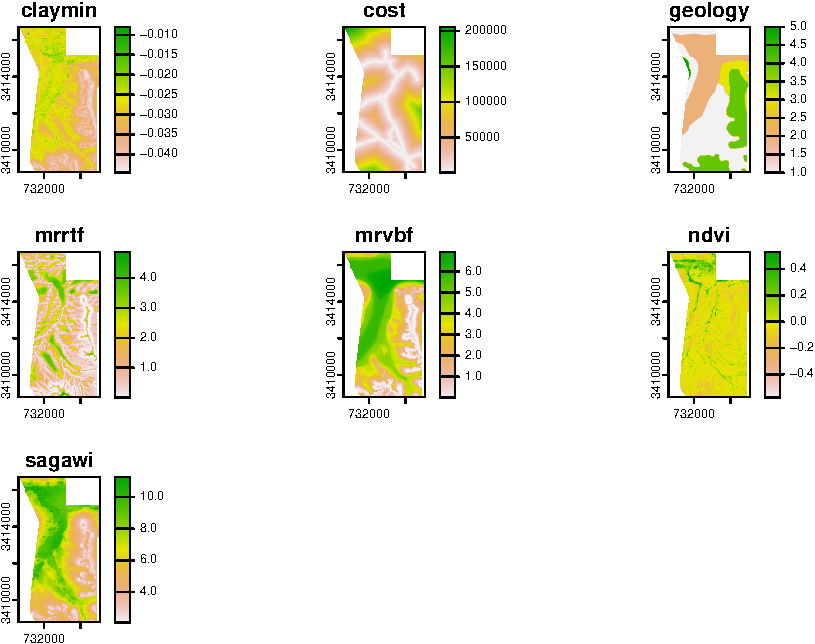
\includegraphics{Technical-Manual-Soil-Sampling-Design_files/figure-latex/fig-3-1.pdf}
\caption{\label{fig:fig-3}Covariates}
\end{figure}

\hypertarget{representativeness-of-the-legacy-soil-data}{%
\section{Representativeness of the Legacy Soil Data}\label{representativeness-of-the-legacy-soil-data}}

The next step involves the determination of the distributions of environmental values in the soil samples data and its comparison with the existing distributions of each environmental variable to determine the representativeness of the soil points in the environmental space.

The comparison of distributions is performed through the Kullback-Leibler divergence (KL). It is a measure used to quantify the difference between two probability distributions.
KL-divergence compares an `objective' or reference probability distribution (here, the distribution of covariates in the complete covariate space - P) with a `model' or approximate probability distribution (the space of covariates in the soil samples - Q). The main idea is to determine how much information is lost when Q is used to approximate P. In other words, KL-divergence measures how much the Q distribution deviates from the P distribution.

We cross soil and environmental data to create a dataset with the values of the environmental parameters at the locations of the soil samples.

\begin{Shaded}
\begin{Highlighting}[]
\CommentTok{\# Extract environmental data from rasters at soil locations {-}{-}{-}{-}}
\NormalTok{  p.dat\_I }\OtherTok{\textless{}{-}}\NormalTok{ terra}\SpecialCharTok{::}\FunctionTok{extract}\NormalTok{(cov.dat, p.dat)}
\NormalTok{  p.dat\_I }\OtherTok{\textless{}{-}} \FunctionTok{na.omit}\NormalTok{(p.dat\_I) }\CommentTok{\# Remove soil points outside study area}
  \FunctionTok{str}\NormalTok{(p.dat\_I)}
\end{Highlighting}
\end{Shaded}

\begin{verbatim}
## 'data.frame':    238 obs. of  5 variables:
##  $ ID       : num  1 2 3 4 5 6 7 8 9 10 ...
##  $ ECd      : num  7.48 5.86 7.4 6.84 6.2 ...
##  $ ECs      : num  7.86 5.67 7.81 6.99 5.51 ...
##  $ elevation: num  127 127 127 127 127 ...
##  $ yield    : num  3.03 3.79 3.37 2.62 3.69 ...
\end{verbatim}

We first calculate a \texttt{\textquotesingle{}n-matrix\textquotesingle{}} with the values of the covariates dividing their distributions into \texttt{\textquotesingle{}n\textquotesingle{}} equally-spaced bins. Each bin captures the environmental variability within its interval in the total distribution. In this exercise, \texttt{\textquotesingle{}n\textquotesingle{}} equals to 25. The result is a 26×4 matrix, where the rows represent the upper and lower limit of the bin and (thus, 26 rows are required to represent 25 bins), and 4 correspond to the number of variables used as environmental proxies.

\begin{Shaded}
\begin{Highlighting}[]
\CommentTok{\# Define Number of bins}
\NormalTok{  nb}\OtherTok{\textless{}{-}} \DecValTok{25}
  \CommentTok{\#quantile matrix (of the covariate data)}
\NormalTok{  q.mat}\OtherTok{\textless{}{-}} \FunctionTok{matrix}\NormalTok{(}\ConstantTok{NA}\NormalTok{, }\AttributeTok{nrow=}\NormalTok{(nb}\SpecialCharTok{+}\DecValTok{1}\NormalTok{), }\AttributeTok{ncol=} \FunctionTok{nlyr}\NormalTok{(cov.dat))}
\NormalTok{  j}\OtherTok{=}\DecValTok{1}
  \ControlFlowTok{for}\NormalTok{ (i }\ControlFlowTok{in} \DecValTok{1}\SpecialCharTok{:}\FunctionTok{nlyr}\NormalTok{(cov.dat))\{ }\CommentTok{\#note the index start here}
  \CommentTok{\#get a quantile matrix together of the covariates}
\NormalTok{    ran1 }\OtherTok{\textless{}{-}} \FunctionTok{minmax}\NormalTok{(cov.dat[[i]])[}\DecValTok{2}\NormalTok{] }\SpecialCharTok{{-}} \FunctionTok{minmax}\NormalTok{(cov.dat[[i]])[}\DecValTok{1}\NormalTok{]}
\NormalTok{    step1}\OtherTok{\textless{}{-}}\NormalTok{ ran1}\SpecialCharTok{/}\NormalTok{nb }
\NormalTok{    q.mat[,j]}\OtherTok{\textless{}{-}} \FunctionTok{seq}\NormalTok{(}\FunctionTok{minmax}\NormalTok{(cov.dat[[i]])[}\DecValTok{1}\NormalTok{], }\AttributeTok{to =} \FunctionTok{minmax}\NormalTok{(cov.dat[[i]])[}\DecValTok{2}\NormalTok{], }\AttributeTok{by =}\NormalTok{step1)}
\NormalTok{    j}\OtherTok{\textless{}{-}}\NormalTok{ j}\SpecialCharTok{+}\DecValTok{1}\NormalTok{\}}
\end{Highlighting}
\end{Shaded}

From this matrix, we compute the hypercube matrix of covariates in the whole covariate space.

\begin{Shaded}
\begin{Highlighting}[]
\CommentTok{\# Hypercube of "objective" distribution (P) {-} covariates}
\NormalTok{  cov.dat.df }\OtherTok{\textless{}{-}} \FunctionTok{as.data.frame}\NormalTok{(cov.dat) }\CommentTok{\# convert SpatRaster to dataframe}
\NormalTok{  cov.mat}\OtherTok{\textless{}{-}} \FunctionTok{matrix}\NormalTok{(}\DecValTok{1}\NormalTok{, }\AttributeTok{nrow=}\NormalTok{nb, }\AttributeTok{ncol=}\FunctionTok{ncol}\NormalTok{(q.mat))}
    \ControlFlowTok{for}\NormalTok{ (i }\ControlFlowTok{in} \DecValTok{1}\SpecialCharTok{:}\FunctionTok{nrow}\NormalTok{(cov.dat.df))\{ }\CommentTok{\# the number of pixels}
\NormalTok{      cntj}\OtherTok{\textless{}{-}} \DecValTok{1} 
    \ControlFlowTok{for}\NormalTok{ (j }\ControlFlowTok{in} \DecValTok{1}\SpecialCharTok{:}\FunctionTok{ncol}\NormalTok{(cov.dat.df))\{ }\CommentTok{\#for each column}
\NormalTok{      dd}\OtherTok{\textless{}{-}}\NormalTok{ cov.dat.df[i,j]  }
      \ControlFlowTok{for}\NormalTok{ (k }\ControlFlowTok{in} \DecValTok{1}\SpecialCharTok{:}\NormalTok{nb)\{  }\CommentTok{\#for each quantile}
\NormalTok{        kl}\OtherTok{\textless{}{-}}\NormalTok{ q.mat[k, cntj] }
\NormalTok{        ku}\OtherTok{\textless{}{-}}\NormalTok{ q.mat[k}\SpecialCharTok{+}\DecValTok{1}\NormalTok{, cntj] }
        \ControlFlowTok{if}\NormalTok{ (}\FunctionTok{is.na}\NormalTok{(dd)) \{}
          \FunctionTok{print}\NormalTok{(}\StringTok{\textquotesingle{}Missing\textquotesingle{}}\NormalTok{)}
\NormalTok{        \}}
        \ControlFlowTok{else} \ControlFlowTok{if}\NormalTok{ (dd }\SpecialCharTok{\textgreater{}=}\NormalTok{ kl }\SpecialCharTok{\&}\NormalTok{ dd }\SpecialCharTok{\textless{}=}\NormalTok{ ku)\{cov.mat[k, cntj]}\OtherTok{\textless{}{-}}\NormalTok{ cov.mat[k, cntj] }\SpecialCharTok{+} \DecValTok{1}\NormalTok{\} }
\NormalTok{      \}}
\NormalTok{      cntj}\OtherTok{\textless{}{-}}\NormalTok{ cntj}\SpecialCharTok{+}\DecValTok{1}
\NormalTok{    \}}
\NormalTok{  \}}
\end{Highlighting}
\end{Shaded}

We then calculate the hypercube matrix of covariates in the sample space.

\begin{Shaded}
\begin{Highlighting}[]
\CommentTok{\# Sample data hypercube}
\NormalTok{  h.mat}\OtherTok{\textless{}{-}} \FunctionTok{matrix}\NormalTok{(}\DecValTok{1}\NormalTok{, }\AttributeTok{nrow=}\NormalTok{nb, }\AttributeTok{ncol=}\FunctionTok{ncol}\NormalTok{(q.mat))}
  
  \ControlFlowTok{for}\NormalTok{ (ii }\ControlFlowTok{in} \DecValTok{1}\SpecialCharTok{:}\FunctionTok{nrow}\NormalTok{(p.dat\_I))\{ }\CommentTok{\# the number of observations}
\NormalTok{    cntj}\OtherTok{\textless{}{-}} \DecValTok{1} 
    \ControlFlowTok{for}\NormalTok{ (jj }\ControlFlowTok{in} \DecValTok{2}\SpecialCharTok{:}\FunctionTok{ncol}\NormalTok{(p.dat\_I))\{ }\CommentTok{\#for each column}
\NormalTok{      dd}\OtherTok{\textless{}{-}}\NormalTok{ p.dat\_I[ii,jj]  }
      \ControlFlowTok{for}\NormalTok{ (kk }\ControlFlowTok{in} \DecValTok{1}\SpecialCharTok{:}\NormalTok{nb)\{  }\CommentTok{\#for each bin}
\NormalTok{        kl}\OtherTok{\textless{}{-}}\NormalTok{ q.mat[kk, cntj] }
\NormalTok{        ku}\OtherTok{\textless{}{-}}\NormalTok{ q.mat[kk}\SpecialCharTok{+}\DecValTok{1}\NormalTok{, cntj] }
        \ControlFlowTok{if}\NormalTok{ (dd }\SpecialCharTok{\textgreater{}=}\NormalTok{ kl }\SpecialCharTok{\&}\NormalTok{ dd }\SpecialCharTok{\textless{}=}\NormalTok{ ku)\{h.mat[kk, cntj]}\OtherTok{\textless{}{-}}\NormalTok{ h.mat[kk, cntj] }\SpecialCharTok{+} \DecValTok{1}\NormalTok{\}}
\NormalTok{      \}}
\NormalTok{      cntj}\OtherTok{\textless{}{-}}\NormalTok{ cntj}\SpecialCharTok{+}\DecValTok{1}
\NormalTok{    \}}
\NormalTok{  \}}
\end{Highlighting}
\end{Shaded}

\begin{itemize}
\tightlist
\item
  \textbf{KL-divergence}
\end{itemize}

We calculate the KL-divergence to measure how much the distribution of covariates in tbe sample space (Q) deviates from the distribution of covariates in the complete study area space (P).

\begin{Shaded}
\begin{Highlighting}[]
\DocumentationTok{\#\# Compare covariate distributions in P and Q with Kullback{-}Leibler (KL) divergence}
\NormalTok{    kl.index }\OtherTok{\textless{}{-}}\FunctionTok{c}\NormalTok{()}
    \ControlFlowTok{for}\NormalTok{(i }\ControlFlowTok{in} \DecValTok{1}\SpecialCharTok{:}\FunctionTok{ncol}\NormalTok{(cov.dat.df))\{}
\NormalTok{      kl }\OtherTok{\textless{}{-}}    \FunctionTok{KL.empirical}\NormalTok{(}\FunctionTok{c}\NormalTok{(cov.mat[,i]), }\FunctionTok{c}\NormalTok{(h.mat[,i]))}
\NormalTok{      kl.index }\OtherTok{\textless{}{-}} \FunctionTok{c}\NormalTok{(kl.index,kl)}
\NormalTok{      klo }\OtherTok{\textless{}{-}}  \FunctionTok{mean}\NormalTok{(kl.index)}
\NormalTok{    \}}
    \FunctionTok{print}\NormalTok{(kl.index) }\CommentTok{\# KL divergences of each covariate}
\end{Highlighting}
\end{Shaded}

\begin{verbatim}
## [1] 0.04115895 0.04241792 0.02779852 0.04328375
\end{verbatim}

\begin{Shaded}
\begin{Highlighting}[]
    \FunctionTok{print}\NormalTok{(klo) }\CommentTok{\# KL divergence in the existing soil samples}
\end{Highlighting}
\end{Shaded}

\begin{verbatim}
## [1] 0.03866478
\end{verbatim}

The KL-divergence is always greater than or equal to zero, and reaches its minimum value (zero) only when P and Q are identical. Thus, lower values of KL-divergence are indicative of a good match between both the sample and the study area spaces, indicating that the sample space is a fair representation of the environmental conditions in the study area.

In this case, the KL-divergence value is 0.039, indicating that the legacy samples capture most of the environmental variability in the study area.

\begin{itemize}
\tightlist
\item
  \textbf{Percent of representativeness in relation to the overall environmental conditions}
\end{itemize}

Finally, we can also determine the degree in which our legacy soil dataset is representative of the existing environmental conditions in the study area. For that, we calculate the proportion of pixels in the study area that would fall within the convex hull polygon delineated upon the environmental conditions found at the soil legacy data locations only. The convex hull polygon is created upon a Principal Component transformation of the covariate data in the soil legacy data and using the outter limits of the scores of the points projected on the two main Components.

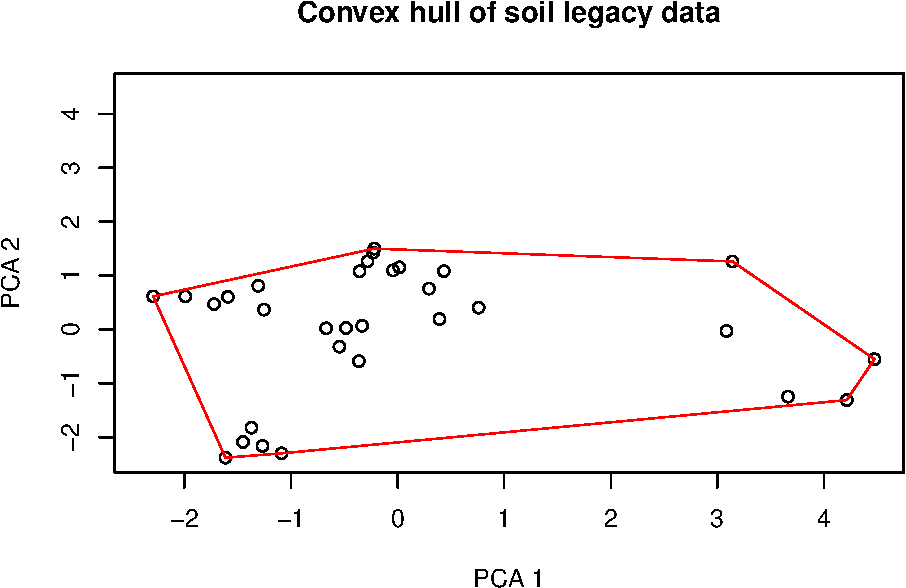
\includegraphics{Technical-Manual-Soil-Sampling-Design_files/figure-latex/fig-4-1.pdf} 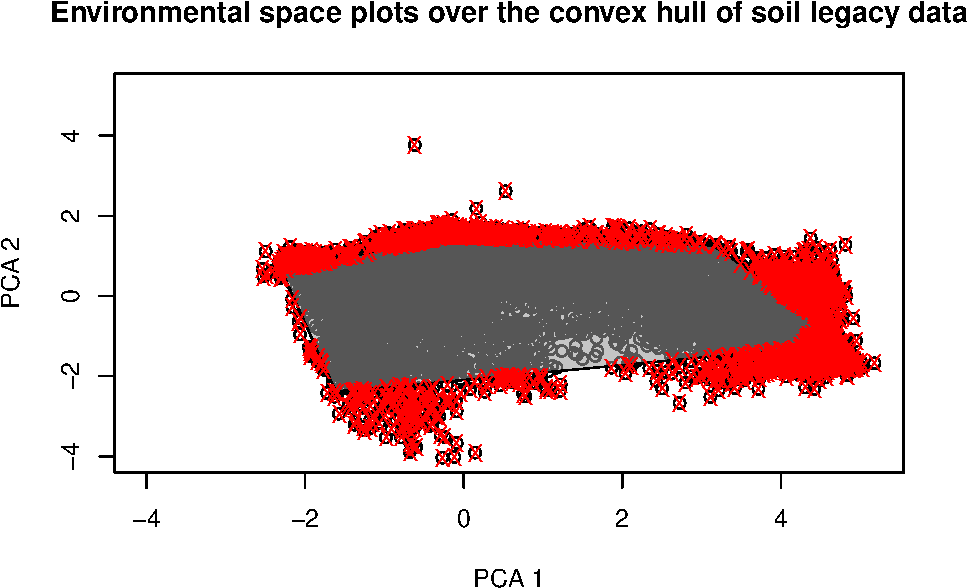
\includegraphics{Technical-Manual-Soil-Sampling-Design_files/figure-latex/fig-4-2.pdf}

\begin{verbatim}
## [1] 96.50188
\end{verbatim}

This indicates that 96.5\% of the existing conditions in the study area fall within the convex hull delineated with the data in the soil samples, showing the adequacy of the proposed legacy data for DSM.

\hypertarget{refs}{}
\begin{CSLReferences}{0}{0}
\leavevmode\vadjust pre{\hypertarget{ref-CLIFFORD201462}{}}%
\textbf{Clifford, D., Payne, J.E., Pringle, M.J., Searle, R. \& Butler, N.} 2014. Pragmatic soil survey design using flexible latin hypercube sampling. \emph{Computers \& Geosciences}, 67: 62--68. \url{https://doi.org/10.1016/j.cageo.2014.03.005}

\leavevmode\vadjust pre{\hypertarget{ref-Malone}{}}%
\textbf{Malone, B.P., Minansy, B. \& Brungard, C.} 2019. Some methods to improve the utility of conditioned latin hypercube sampling. \emph{PeerJ}, 7: e6451. \url{https://doi.org/10.7717/peerj.6451}

\leavevmode\vadjust pre{\hypertarget{ref-minasny2006}{}}%
\textbf{Minasny, B. \& Mcbratney, A.} 2006. A conditioned latin hypercube method for sampling in the presence of ancillary information. \emph{Computers \& Geosciences}, 32: 1378--1388. \url{https://doi.org/10.1016/j.cageo.2005.12.009}

\leavevmode\vadjust pre{\hypertarget{ref-SENA2021e00354}{}}%
\textbf{Sena, N.C., Veloso, G.V., Lopes, A.O., Francelino, M.R., Fernandes-Filho, E.I., Senra, E.O., Silva Filho, L.A. da, Condé, V.F., Arruda Silva, D.L. de \& Araújo, R.W. de}. 2021. Soil sampling strategy in areas of difficult acess using the cLHS method. \emph{Geoderma Regional}, 24: e00354. \url{https://doi.org/10.1016/j.geodrs.2020.e00354}

\end{CSLReferences}

\end{document}
